\chapter{Arrays}
	\label{ch:arrays}

	This chapter explains:
	\begin{itemize}
    \item how to declare an array;
    \item how to use an index;
    \item how to obtain the size of an array;
    \item how to use \keyword{ReDim};
    \item how to pass arrays as parameters;
    \item how to initialize an array;
    \item how to carry out typical operations such as lookup and searching;
    \item how to create arrays of objects.
	\end{itemize}


  \section{Introduction}
		So far in this book, we have described data items (variables) that are individual and isolated. For example:
		\begin{lstlisting}
Dim count, sum As Integer
Dim name As String
		\end{lstlisting}
		These live on their own, performing useful roles in programs as counters, sums or whatever. We can think of these variables as places in memory that have individual names attached to them.
		
		In contrast, we very often in life deal with data that is not isolated, but grouped together into a collection of information. Sometimes the information is in tables. Examples are a train timetable, a telephone directory or a bank statement. In programming, these things are called data structures. The information in a table is related in some way to the other information within the table. One of the simplest types of data structure in programming is an array. An array can be regarded simply as a table, with a single row of information. (Alternatively you can visualize a table as a single column of information.) This could be a table of numbers, a table of strings or a table of anything.
		
		In this chapter we will look at arrays of numbers, arrays of strings and arrays of other objects, such as graphical objects.
		
		Here is an array of numbers:
		\begin{center}
			\begin{tabular}{|l|l|l|l|l|l|l|}
				\hline 2& 3	&54&	96&	13&	7&	32 \\ \hline
			\end{tabular}
		\end{center}
		which might represent the ages of a group of people at a party. And here is a table of words, which holds the names of the members of a band:
		\begin{center}
			\begin{tabular}{|l|l|l|l|}
				\hline John&	Paul&	George &	Ringo\\ \hline
			\end{tabular}
		\end{center}
		In VB, a table like this is called an array. In programming, an item in an array is known as an \emph{element} and we refer to an element by its position in the array, called the \emph{index}. (In the world of programming, the term \emph{component} is sometimes used instead of element, and the term \emph{subscript} instead of index.) To us humans, the name John is in the first position in this table, but in VB the first position in an array is called the zeroth position. Successive positions in an array are the zeroth, first, second, third, etc. Thus the string Ringo is in the third position in the above array. The position of an element in an array is called the index. We can therefore picture an array, together with its indices, like this:
		\begin{center}
			\begin{tabular}{l |l|l|l|l|}
				\cline{2-5}
				array: &	John	&Paul&	George&	Ringo\\ \cline{2-5}
			\multicolumn{1}{l}{indices:} &	\multicolumn{1}{l}{0} &	\multicolumn{1}{l}{1} &	\multicolumn{1}{l}{2}  &	\multicolumn{1}{l}{3} 
			\end{tabular}
		\end{center}

Remember that the indices are not held in the computer's memory – only the data. The indices are the way that we locate information in an array.
Here is another array, this time containing numbers. The indices for the array are also shown:
		\begin{center}
			\begin{tabular}{l |l|l|l|l|l|l|}
				\cline{2-7}
				array: &	23 &	54 &	96&	13 &	7 &	32 \\ \cline{2-7}
			\multicolumn{1}{l}{indices:} &	\multicolumn{1}{l}{0} &	\multicolumn{1}{l}{1} &	\multicolumn{1}{l}{2}  &	\multicolumn{1}{l}{3} &\multicolumn{1}{l}{4} & \multicolumn{1}{l}{5}  
			\end{tabular}
		\end{center}
		In a program (as in real life) we typically have to carry out the following operations on arrays:
		\begin{itemize}
      \item Create the array – say how long it is and what sort of things it will contain.
      \item Put some values in the array (for example, enter some numbers into a personal telephone directory).
      \item Display the contents of the array on the screen (an array is held in the computer's memory and it is therefore invisible).
      \item Search the array to find some value (for example, searching the train timetable to find a train at a convenient time).
      \item Add up the contents of the array (for example, working out how much a customer spent at the supermarket).
		\end{itemize}
		During this chapter we shall see how to carry out these actions one by one and build up to doing all these things in a complete program. We shall start by looking at arrays of numbers. Our plan is to develop a program with the screen layout shown later in \Vref{fig:arrays_rainfall_screen}. An array holds the data on the rainfall for the seven days in a week (Monday to Sunday.) The user of the program can change the value of any individual data item in the array. The largest of the numbers in the array is to be displayed.


	\section{Creating an array}
		In VB, an array is declared just like any other variable, usually either at the top of a class or at the top of a method. The programmer gives the array a name, like this:
		\begin{lstlisting}
Dim ages(5) As Integer
Dim band(3) As String
		\end{lstlisting}
		The variable named \keyword{ages} is now ready to hold an array of integers. As with any other variable, it is usual (and a good idea) to choose a name for the array that describes clearly what it is going to be used for. The name is the name for the complete array – the complete collection of data. The rules for choosing the name of an array are the same as for choosing any other variable name in VB. The number in brackets after the array name is the value of the largest index.
		\begin{itemize}
			\item The array called \keyword{ages} is big enough to contain six numbers, with indices going from 0 to 5.
			\item The array called \keyword{band} is big enough to contain four strings. The indices go from 0 to 3.
		\end{itemize}

		\begin{stqb}
			\begin{STQ}
				\item	Declare an array to hold data for the rainfall for each of the seven days of the week.
			\end{STQ}
		\end{stqb}


	\section{Indices}
	The way that a program refers to an individual item in an array is to specify an index value (sometimes called a subscript). Thus \keyword{ages(3)} refers to the element in the array with index 3 – the value 12 in this case. Similarly, \keyword{band(2)} contains the string \keyword{George}. Remember that indices start at 0, so an array of length 4 has indices that go from 0 to 3. Therefore a reference to \keyword{band(4)} is an error. The program will stop and an error message will be displayed.
		
		In summary, index values:
		\begin{itemize}
      \item start at zero;
      \item are integers;
      \item go up to the value specified when the array is declared.
		\end{itemize}
		Sometimes, as we shall see, it is useful to use a variable value as an index. In such cases, it is usual to use \keyword{Integer} variables as indices.
		
		We can input a value for an element of an array using a text box:
		\begin{lstlisting}
ages(2) = CInt(TextBox1.Text)
band(3) = TextBox2.Text
		\end{lstlisting}
		and similarly output values:
		\begin{lstlisting}
TextBox3.Text = "the first age is " & CStr(ages(0))
TextBox4.Text = "the 4th band member is " & band(3)
		\end{lstlisting}
		This latter example shows how careful you have to be with array indices.
		
		You can change the values of individual elements of an array with assignments statements, like this:
		\begin{lstlisting}
ages(3) = 99
band(2) = "Mike"
		\end{lstlisting}
		In all these program fragments, we are referring to individual elements in an array by specifying the value of a index.

		\begin{stqb}
			\begin{STQ}
				\item	Given the declaration:
					\begin{lstlisting}
Dim table(2) As Integer
					\end{lstlisting}
					how long is the array and what is the valid range of indices?
			\end{STQ}
		\end{stqb}

		Very often we want to refer to the \emph{n}th element in an array, where \emph{n} is a variable. This is how the power of arrays really comes into its own. Suppose, for example, we want to add up all the numbers in an array (of numbers). Let us suppose that we have an array with seven elements that hold the number of computers sold in a shop during each day in a week:
		\begin{lstlisting}
Dim sale(6) As Integer
		\end{lstlisting}
		We will insert values into the array with assignment statements. Suppose that on Monday (day 0), 13 computers are sold:
		\begin{lstlisting}
sale(0) = 13
		\end{lstlisting}
		and so on for the other days
		\begin{lstlisting}
sale(1) = 8
sale(2) = 22
sale(3) = 17
sale(4) = 24
sale(5) = 15
sale(6) = 23
		\end{lstlisting}
		Next we want to find the total sales for the week. The clumsy way to add up the sales would be to write:
		\begin{lstlisting}
sum = sale(0) + sale(1) + sale(2) + sale(3) + sale(4) + sale(5) + sale(6)
		\end{lstlisting}
		which is quite correct, but does not exploit the regularity of an array. The alternative is to use a \keyword{For} loop. A variable called, say, \keyword{dayNumber} is used to hold the value of the index representing the day of the week. The index is made initially equal to 0 and then incremented each time the loop is repeated:
		\begin{lstlisting}
Dim sum As Integer
Dim dayNumber As Integer
sum = 0
For dayNumber = 0 To 6
	sum = sum + sale(dayNumber)
Next
		\end{lstlisting}
		Each time the loop is repeated, the next value in the array is added to the total. This program fragment is actually no shorter than what it replaces. But it would be considerably shorter if the array had 1000 items to add up! The other advantage is that the code explicitly shows that it is performing a systematic operation on an array.
		
		Indices are the one place in programming when it is permissible (sometimes) to use a name that is a little cryptic. In the above program fragment, however, using the name \keyword{dayNumber} as the index is clear and relates strongly to the problem being solved.

		\begin{stqb}
			\begin{STQ}
				\item	What does the following program fragment do?
					\begin{lstlisting}
Dim table(9) As Integer
Dim index As Integer
For index = 0 To 10
	table(index) = index
Next
					\end{lstlisting}
			\end{STQ}
		\end{stqb}


	\section{The length of an array}
		A running program can always find out how long an array is. For example if we have an array declared like this:
		\begin{lstlisting}
Dim table(9) As Integer
		\end{lstlisting}
		we can access its length by making use of the function \keyword{UBound} (short for upper bound) like this:
		\begin{lstlisting}
Dim length As Integer
length = UBound(table)
		\end{lstlisting}
		\keyword{UBound} means the largest valid index (9 in this case). We shall see that this facility is very useful.

		Once you have created an array, its length is fixed. Arrays are not made of elastic – an array will not expand as necessary to hold information – but an array can be rebuilt to a different size. This is accomplished using the \keyword{ReDim} statement. For example, suppose we have an array:
		\begin{lstlisting}
Dim table(19) As Integer
		\end{lstlisting}
		Then we can change its size when the program runs by:
		\begin{lstlisting}
ReDim table(39)
		\end{lstlisting}
		We can even declare an array with no size, then specify its size later. For example:
		\begin{lstlisting}
Dim table() As Integer
ReDim table(24)
		\end{lstlisting}
		Doing a \keyword{ReDim} destroys the data in the array. But it can be preserved using Preserve as follows:

		\begin{lstlisting}
ReDim Preserve table(24)
		\end{lstlisting}
		When you design a new program, you need to consider how big any array should be. This is sometimes obvious from the nature of the problem. For example, if the data relates to the days of the week, then you know that the array needs seven elements. On some occasions, the size of the array needs to be flexible, and this is where \keyword{ReDim} comes in useful. However, there are other types of data structure (such as an array list) that expand and contract bit by bit as needed.


	\section{Passing arrays as parameters}
		As we have seen in earlier chapters of this book, methods are very important in programming. An important aspect of using methods is passing information as parameters and returning a value. We now explain how to pass and return arrays.
		
		Suppose we want to write a method whose job it is to calculate the sum of the elements in an array of integers. Being perceptive programmers, we want the method to be general-purpose, so that it will cope with arrays of any length. But that is OK because the method can easily find out the length of the array. So the parameter to be passed to the method is simply the array and the result to be returned to the user of the method is a number, the sum of the values.
		
		A sample call of the method looks like this:
		\begin{lstlisting}
Dim table(23) As Integer
Dim total As Integer
total = Sum(table)
		\end{lstlisting}
		The method itself is:
		\begin{lstlisting}
Private Function Sum(array() As Integer) As Integer
	Dim total As Integer
	Dim index As Integer
	total = 0
	For index = 0 To UBound(array)
		total = total + array(index)
	Next
	Return total
End Function
		\end{lstlisting}
		
		Notice that in the header for the method the parameter is declared as an array, with brackets. But there is no parameter that spells out how long the array actually is. The method finds out the value of the largest index using the method \keyword{UBound}. Because it will accept an array of any length, this method is general purpose and potentially very useful. This is highly preferable to a special-purpose method that will only work when the array is, say, eight elements long.
		
		\begin{stqb}
			\begin{STQ}
			\item Write a method that displays an array of integers, one per line, in a multiline text box. The single parameter to the method is the array.
			\end{STQ}
		\end{stqb}


	\section{The \keyword{For Each} statement}
		It is very common to use \keyword{For} statements in conjunction with arrays. But on those occasions that the program needs to process every item in an array, there is a neat way of doing it using the \keyword{For Each} statement. We can rewrite the above method to calculate the sum of the integers in an array, as follows:
		\begin{lstlisting}
Private Function Sum(array() As Integer) As Integer
	Dim total As Integer
	total = 0
	For Each n As Integer In array
		total = total + n
	Next
	Return total
End Function
		\end{lstlisting}
		You will see that it is much neater and shorter. The \keyword{For} statement can be read as ‘for each integer \keyword{n} in the array'. The loop is repeated for all the elements of the array. At each repetition, the variable \keyword{n} holds the value of the element in the array.

		The type declared as part of the \keyword{For} statement (\keyword{Integer} in this example) must match with the type that the array holds. The variable (\keyword{n} in this example) can have any name, just like any other variable.
		
		There are three things to remember when you are contemplating using a \keyword{For Each} statement:
		\begin{itemize}
      \item You can only use the \keyword{For Each} statement when you need to process all the items in an array.
      \item Inside the loop, the index value is not available.
      \item You cannot change the value of an array element using the \keyword{For Each}.
		\end{itemize}
		For these reasons you will see that only a small number of the programs in this chapter use \keyword{For Each}.


	\section{Using constants}
		In a program with several arrays, there are declarations of the arrays and almost certainly lots of \keyword{For} loops. The arrays, together with their lengths, will be passed around the program as parameters. There is plenty of scope for confusion, particularly if two different arrays have the same length.
		
		Suppose, for example, we are writing a program to analyse marks that students obtain in assignments. Suppose there are 10 students. We want one array to hold the average mark for each student:
		\begin{lstlisting}
Dim studentMark(9) As Integer
		\end{lstlisting}
		By coincidence, there are also 10 courses. We also want a second array to hold the average mark for each course:
		\begin{lstlisting}
Dim courseMark(9) As Integer
		\end{lstlisting}
		The problem is that, wherever we see the number 9 in the program, we do not know whether it is the number of students minus 1 or it is the number of courses minus 1. As things stand, of course, it does not matter – because they are the same! But suppose we needed to alter the program so that it deals with 20 students. We would very much like to change every occurrence of the number 9 to the number 19 using the replace function within the Integrated Development Environment. But because the arrays are the same length, this would cause great damage to the program.
		
		One way to clarify such a program is to declare the lengths of the arrays as constants, and then to use the constants in \keyword{For} loops like this:
		\begin{lstlisting}
Const students As Integer = 19
Const courses As Integer = 24
Then we can use the constants as follows:
Dim studentMark(students) As Integer
Dim courseMark(courses) As Integer
Dim index As Integer
For index = 0 To students
' body of loop
Next
		\end{lstlisting}
		We can now make changes to the program with complete confidence, simply by changing a single number in the constant declaration.

		\begin{stqb}
			\begin{STQ}
				\item Write the code to place zeroes in every element of the array \keyword{courseMark}.
			\end{STQ}
		\end{stqb}


	\section{Initializing an array}
		Initializing means giving a variable an initial or starting value. If you write this:
		\begin{lstlisting}
Dim table(9) As Integer
		\end{lstlisting}
		then an array is set up in memory and the array contains zeroes. When the programmer does not explicitly give initial values, the compiler inserts default values. These are zeroes for numbers, "" for strings and \keyword{Nothing} for objects.

		A common way of explicitly initializing an array is to do it when the array is declared. The required initial values are enclosed in curly brackets and separated by commas. But the size of the array must not be given in its usual place. The following initialization:
		\begin{lstlisting}
Dim ages() As Integer = {23, 54, 96, 13, 7, 32}
is equivalent to:
Dim ages(5) As Integer
ages(0) = 23
ages(1) = 54
ages(2) = 96
ages(3) = 13
ages(4) = 7
ages(5) = 32
		\end{lstlisting}
		Here is another example, initializing an array of strings:
		\begin{lstlisting}
Dim band() As String = {"John", "Paul", "George", "Ringo"}
		\end{lstlisting}
		Another way to initialize an array is to use a loop as we saw earlier, like this:
		\begin{lstlisting}
Dim table(25) As Integer
Dim index As Integer
For index = 0 To UBound(table)
    table(index) = 0
Next
		\end{lstlisting}
		If the program needs periodically to reset the array back to its initial values, then the way to do it is by using the \keyword{For} loop as shown above.

		\begin{stqb}
			\begin{STQ}
				\item	Declare an array called \keyword{numbers} of 5 integers and fill it with the numbers 1 to 5 as part of the declaration.
			\end{STQ}
		\end{stqb}


	\section{A sample program}
		Now we will combine all the things we have explained into a program to input some numbers, put them in an array and display them. The screen is shown in \Vref{fig:arrays_rainfall_screen}. The data displayed represents the rainfall for the seven days in a week (Monday to Sunday). The user of the program enters values into a text box to say which index value and a text box to provide the rainfall value for that day. The largest of the rainfall values is displayed.
		\begin{figure}[bth]
			\centering
			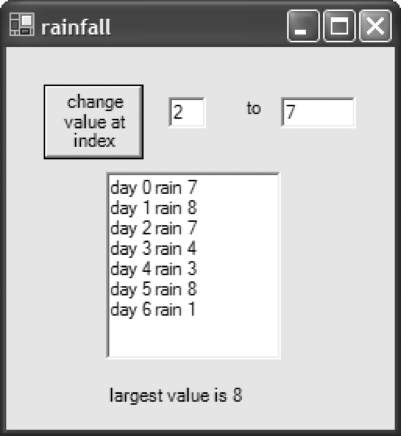
\includegraphics[width=7cm]{arrays_rainfall_screen}
			\caption{The display from the rainfall program.}
			\label{fig:arrays_rainfall_screen}
		\end{figure}

		
		First, the array is declared at the top of the form class. It has its values initialized to a selection of values.
		\begin{lstlisting}
Private rain() As Integer = {7, 8, 7, 4, 3, 8, 1}
		\end{lstlisting}
Next the code to display the array values in a multiline text box:
		\begin{lstlisting}
Private Sub Display()
	Dim daynumber As Integer
	RainfallTextBox.Clear()
	For daynumber = 0 To 6
		RainfallTextBox.AppendText("day " & CStr(daynumber)
			& " rain " & CStr(rain(daynumber))
			& NewLine)
	Next
End Sub
		\end{lstlisting}
		Next we look at the code to place a new value in an element of the array. The index value is in one text box; the actual value of the data in another. Finally the method \keyword{Display} is called to display the updated value, and \keyword{Largest} is called to display the largest value.
		\begin{lstlisting}
Private Sub NewValue()
	Dim index As Integer
	Dim data As Integer
	index = CInt(IndexTextBox.Text)
	data = CInt(ValueTextBox.Text)
	rain(index) = data
	Display()
	Largest()
End Sub
		\end{lstlisting}
		We now look at the code to calculate the largest rainfall value. The approach used is to start by assuming that the first item is the largest. Then we look at the remainder of the elements in turn, comparing them with this largest value. If we find a value that is larger than the one we have already got, we update our largest value. This is a classic approach.
		\begin{lstlisting}
Private Sub Largest()
	Dim highest As Integer
	Dim index As Integer
	highest = rain(0)
	For index = 0 To 6
		If highest < rain(index) Then
			highest = rain(index)
		End If
	Next
	LargestLabel.Text = "largest value is " & CStr(highest)
End Sub
		\end{lstlisting}
		You will see that it is very common to use the \keyword{For} statement in conjunction with arrays. They go together like a horse and carriage, in the words of the song. It is, of course, because a \keyword{For} loop makes the maximum use of the uniformity of arrays.

		\begin{stqb}
			\begin{STQ}
			\item Write a method to calculate and display the total rainfall for the week.
			\end{STQ}
		\end{stqb}



	\section{Lookup}
		Part of the power of arrays is that you can look up something very easily and quickly. In the rainfall program, we can extract the value of Tuesday's rainfall simply by referring to rain(1). The same is true of any information that can be referred to by an integer index. For example, if we have a table showing the average height of people according to age, we can index the table using an age (25 in this example):
		\begin{lstlisting}
Dim height(99) As Double
Dim myHeight As Double
myHeight = height(25)
		\end{lstlisting}
Similarly, if we have numbered the days of the week as 0 to 6, we can convert a number to a text string like this:
		\begin{lstlisting}
Dim dayNumber As Integer
Dim dayName As String
Dim name() As String =
	{"Monday", "Tuesday", "Wednesday", "Thursday",
		"Friday", "Saturday", "Sunday"}
dayName = name(dayNumber)
		\end{lstlisting}
		This could be accomplished in another way, using a \keyword{Select} statement, which is slightly longer and probably more cumbersome.
		
		Using an array to look up something is extremely useful, simple and exploits the power of arrays.

		\begin{stqb}
			\begin{STQ}
				\item Rewrite the above conversion using a \keyword{Select} statement.
			\end{STQ}
		\end{stqb}


	\section{Searching}
	Another way of accessing information in an array is to search for it. This is what humans do in a telephone directory or a dictionary. The example we will consider is a telephone directory (\Vref{fig:arrays_telephone_screen}).
		\begin{figure}[bth]
			\centering
			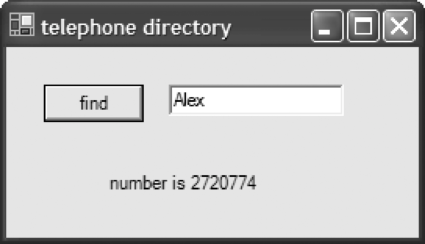
\includegraphics[width=6cm]{arrays_telephone_screen}
			\caption{The display from the rainfall program.}
			\label{fig:arrays_telephone_screen}
		\end{figure}

		We will set up two arrays, one to hold names and one to hold the equivalent telephone numbers:
		\begin{lstlisting}
Private names(20) As String
Private numbers(20) As String
		\end{lstlisting}
		Now that the arrays have been created, we can place some data in them:
		\begin{lstlisting}
names(0) = "Alex"
numbers(0) = "2720774"
names(1) = "Megan"
numbers(1) = "5678554"
names(2) = "END"
		\end{lstlisting}
		A simple and effective way to search the directory is to start at the beginning and go from one entry to the next until we find the name that we are looking for. However, the name we seek might not be in the directory, and we must cater for that situation arising. So the search continues until either we find what we are looking for or we get to the end of the entries. We could check that we have got to the end of the array, but a more convenient approach is to put a special entry into the array to signify the end of the useful data. This end marker will consist of an entry with the name \keyword{END}.
		
		Now we can write the loop to search for a desired telephone number.
		\begin{lstlisting}
Private Sub Find()
	Dim index As Integer
	Dim wanted As String
	wanted = TextBox1.Text
	index = 0
	Do Until names(index) = wanted
			Or
		names(index) = "END"
		index = index + 1
	Loop
	If names(index) = wanted Then
		Label1.Text = "number is " & numbers(index)
	Else
		Label1.Text = "name not found"
	End If
End Sub
		\end{lstlisting}
		This is called a \emph{serial} search. It starts at the beginning of the array, with the index zero, and continues searching item-by-item, adding one to the index. The search continues until either the wanted item is found or until the special name \keyword{END} is reached. The most convenient way of controlling this loop is to use a \keyword{Do Until} statement as shown. This repeats until the condition is \keyword{True}.
		
		This type of search makes no assumptions about the order of the items in the table – they can be in any order. Other search techniques exploit the ordering of items in tables, such as alphabetical ordering. These techniques are beyond the scope of this book.
		
		Information like telephone numbers is normally stored in a file, rather than an array, because data held in a file is more permanent. Usually the file is searched for the required information rather than an array. Alternatively, the file is input into memory, held in an array and searched as shown above.


	\section{Arrays of objects}
		Arrays can hold anything – integers, floating-point numbers, strings, buttons, track bars, any object in the library, or any object that the programmer constructs. The only constraint is that all the objects in an array must be of the same type. We will create an array of balloon objects (\Vref{fig:arrays_balloons_screen}). We introduced the balloon object earlier in this book.
		\begin{figure}[bth]
			\centering
			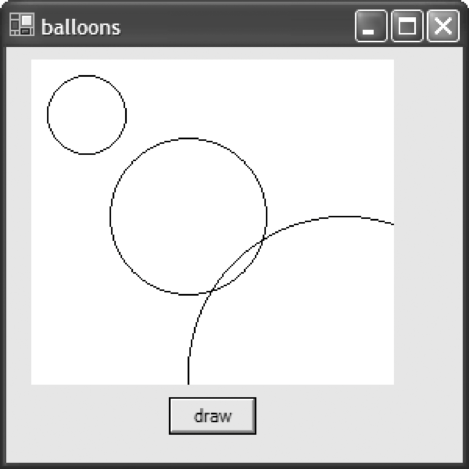
\includegraphics[width=7cm]{arrays_balloons_screen}
			\caption{Drawing an array of balloons.}
			\label{fig:arrays_balloons_screen}
		\end{figure}


		A balloon object (really just a circle) has a size and a position on the screen. Methods are provided as part of the object to move it, change its size and display it. Here is the class:
		\begin{lstlisting}
Public Class Balloon
	Private x As Integer
	Private y As Integer
	Private diameter As Integer
	Public Sub New(initialX As Integer,
			initialY As Integer,
			initialDiameter As Integer)
		MyBase.New()
		x = initialX
		y = initialY
		diameter = initialDiameter
	End Sub
	Public Sub ChangeSize(change As Integer)
		diameter = diameter + change
	End Sub
	Public Sub Display(drawArea As Graphics,
				myPen As Pen)
		drawArea.DrawEllipse(myPen, x, y, diameter, diameter)
	End Sub
End Class
		\end{lstlisting}
		We can now create an array of balloons:
		\begin{lstlisting}
Private party(10) As Balloon
		\end{lstlisting}
		But this only creates the array, ready to hold balloons. We now need to create some balloons as follows:
		\begin{lstlisting}
party(0) = New Balloon(10, 10, 50)
party(1) = New Balloon(50, 50, 100)
party(2) = New Balloon(100, 100, 200)
		\end{lstlisting}
		and display all the balloons:
		\begin{lstlisting}
Private Sub DisplayBalloons()
	Dim b As Integer
	drawArea.Clear(Color.White)
	For b = 0 To 2
		party(b).Display(drawArea, myPen)
	Next
End Sub
		\end{lstlisting}
		The advantage of storing the balloon objects in an array is that we can do something with them all in convenient way. For example, we can change the size of all the balloons at once:
		\begin{lstlisting}
For b = 0 To 2
	party(b).ChangeSize(20)
Next
		\end{lstlisting}
		Finally, we have said that all the elements in an array must be of the same type. There is an exception: if you declare an array of objects of the class \keyword{Object}, then you can place different types of objects in the array. This is because \keyword{Object} is the superclass of every other class.


	\section{Programming principles}
		\begin{itemize}	
			\item An array is a collection of data with a single name. All the items in an array are of the same type. Individual elements in an array are identified by means of an index, an integer. So if for example an array is named \keyword{table}, an individual element is referred to as \keyword{table(2)}, where 2 is the index. You can similarly refer to an element of an array using a integer variable as an index, like \keyword{table(index)}. It is this facility that makes arrays powerful.
      \item Once created, an array has a length and normally this length stays fixed. But the length can be changed as the program executes using \keyword{ReDim}, although this would be carried out at strategic times, rather than frequently.
      \item Arrays can hold data of any type – for example \keyword{Integer}, \keyword{Double}, \keyword{Boolean}, \keyword{Button}, \keyword{TextBox}. (But in any one array the data must all be of the same type.) 
      \item The array is the oldest and most widely used data structure. Arrays are compact and are accessed very quickly using support from the computer's instructions.
      \item It is common to use the \keyword{For} loop in conjunction with arrays.
		\end{itemize}


	\section{Programming pitfalls}
		A common error in VB is to confuse the length of an array with the range of valid indices. For example, the array:
		\begin{lstlisting}
Dim table(9) As Integer
		\end{lstlisting}
		has 10 elements. The valid range of indices for this array is 0 to 9. Reference to \keyword{table(10)} is a reference to an element of the array that simply does not exist. Luckily the VB system checks for violations like this as the program is running and will issue an error message.
		
		Here is a common example of how to do things wrongly:
		\begin{lstlisting}
Dim table(9) As Integer
Dim index As Integer
For index = 0 To 10   ‘warning, erroneous
	table(index) = 0
Next
		\end{lstlisting}
		This will place a zero in all of the elements of the array \keyword{table}, but then go on to try to place a zero in whatever data item happens to be immediately after the array in the computer's memory. The program then fails with an '\keyword{IndexOutOfRange}' message. It is always worthwhile carefully checking the condition for terminating a \keyword{For} loop used with an array.
		
		Students sometimes have difficulty in visualizing where an array is. An array is held in main memory; it is invisible; it only has a life while the program is running.


	\section{Grammar spot}
		An array with 21 elements is declared like this:
		\begin{lstlisting}
Dim table(20) As Double
		\end{lstlisting}
		To refer to an element of an array, the index is written in brackets, as in:
		\begin{lstlisting}
table(3) = 12.34
		\end{lstlisting}


	\section{Summary}
		\begin{itemize}
      \item An array is a collection of data. It is given a name by the programmer. All the items in an array must be of the same type (e.g. all \keyword{Integer}).
      \item An array is declared, along with other variables, like this:
				\begin{lstlisting}
Dim harry(24) As Integer
				\end{lstlisting}
				in which 24 is the value of the largest index. The array has 25 elements.
      \item An individual element in an array is referred to by an integer index, for example:
				\begin{lstlisting}
harry(12) = 45
				\end{lstlisting}
      \item Indices have values that start from zero and go up to the largest index value.
		\end{itemize}


		\section{Exercises}
%\begin{extract*}
			Games
			\begin{EXE}
				\item \name{Nim} The human plays against the computer. At the start of the game there are three piles of matches. In each pile there is a random number of matches in the range 1 to 20. The three piles are displayed throughout the game. A random choice determines who goes first. Players take it in turns to remove as many matches as they like from any one pile, but only from one pile. A player must remove at least one match. The winner is the player who makes the other player take the last match. Make the computer play randomly, that is, it chooses a pile randomly and then a number of matches randomly from those available.
				\item	\name{Safe combination} Set up an array to contain the six digits that open a safe. Ask the user to input six digits one-by-one from buttons labelled with the digits 0 to 9, and check whether they are correct. When a digit is entered, tell the user whether it is correct or not and give them three tries before making them start from the beginning again.
				\item \name{Pontoon (vingt-et-un)} Write a program to play this card game. The computer acts as the dealer. The dealer first deals you two playing cards. These are random cards. (In the real game, the dealer has an enormous hand of cards, comprising several shuffled packs.) Your aim is to get a score higher than the dealer's, without going beyond 21 (vingt-et-un). Ace counts either as 1 or 11. At any time, you can say ‘twist', which means that you want another card, or ‘stick', which means you are content with what you have. You may also have gone ‘bust', which means you have more than 21. When you finally stick or bust, it is the dealer's turn to deal cards for him- or herself. The dealer's aim is to get a bigger score than you, without going bust. But the dealer does not know your score and so gambles on what you might have.
				
					Provide buttons to start a new game, twist and stick. Display both sets of cards that are dealt.
			\end{EXE}

			Basic operations on arrays
			\begin{EXE}
			\item	\name{Rain data} Complete the program to handle rainfall data by including the following operations:
					\begin{itemize}
			      \item Add up the values and display the total.
			      \item Find the largest value, the smallest value and display them.
     			 	\item Find the index of the largest value.
					\end{itemize}
				\item	\name{String array} Write a program that uses an array of 10 strings. Write methods that carry out each of the following operations:
					\begin{itemize}
						\item Input values from the keyboard via a text box.
			      \item Display the values. (You can now observe that they have been entered correctly into your array.)
      			\item Input a word from a text box and search to see whether it is present in the array. Display a message to say whether it is present in the array or not.
					\end{itemize}
				\item	\name{Bar chart} Bar charts are useful for data like rainfall or changes in house prices. Write a method that displays a bar chart of the data that is passed to it as an array. The array holds a number of values, such as the rainfall on each of the seven days of the week. The library method \keyword{FillRectangle} can be used to draw individual bars.
				\item	\name{Pie chart} Pie charts show the proportions of quantities and are therefore useful for data like personal budgets or company budgets. Write a method that displays a pie chart of the data that is passed to it as an array. The array holds the amounts spent on, for example, travel, food, housing, etc. Investigate the \keyword{FillPie} method.
				\item	\name{Graph drawer} Write a method to draw a graph of a data given as an array of x-coordinates and an array of corresponding y-coordinates. It has the heading:
					\begin{lstlisting}
Private Sub DrawGraph(x() As Double, y() As Double)
					\end{lstlisting}
					The method draws straight lines from one point to another. It also draws the axes.
			\end{EXE}

			Statistics
			\begin{EXE}
				\item	Write a program that inputs a series of integers into an array. The numbers are in the range 0 to 100.
					Calculate and display:
					\begin{itemize}
			      \item the largest number;
      			\item the smallest number;
			      \item the sum of the numbers;
			      \item the mean of the numbers.
					\end{itemize}
					Display a histogram (bar chart) that shows how many numbers are in the ranges 0 to 9, 10 to 19, etc.
			\end{EXE}
			
			Random numbers
			\begin{EXE}
				\item	Check to see that the random number generator class (\Cref{ch:objects}) works correctly. Set it up to provide random numbers in the range 1 to 100. Then call the method 100 times, placing the frequencies in an array as in the last exercise. Finally, display the frequency histogram, again as in the last exercise. Random numbers should be random, so the histogram should have bars of approximately equal height.
			\end{EXE}
			
			Words
			\begin{EXE}
			\item	\name{Word perm} Write a program that inputs four words and then displays all possible permutations of the words. So, for example, if the words mad, dog, bites and man are entered, then the following are output:
					\begin{quote}
						man bites mad dog
						mad man bites dog
						mad bites man dog
						etc.
					\end{quote}
					(Not all of the sentences will make sense!)
			\end{EXE}
			
			Information processing – searching
			\begin{EXE}
				\item \name{Dictionary} Set up an array to contain pairs of equivalent English and Spanish words. Then input an English word, look up its Spanish equivalent and display it. Make sure you check to see whether the word is in the dictionary. Then add the facility to translate in the opposite direction, using the same data.
				\item	\name{Library} Each member of a library has a unique user code, an integer. When someone wants to borrow a book, a check is made that the user code is valid.
					Write a program that searches a table of user codes to find a particular code. The program should display a message saying that the code is either valid or invalid.
				\item	\name{Telephone directory} Enhance the telephone directory program given above within the chapter so that new names and numbers can be added to the directory. Then add the facility to remove a name and number.
			\end{EXE}
			
			Information processing – sorting
			\begin{EXE}
				\item	\name{Sorting} Write a program that inputs a series of numbers, sorts them into ascending numerical order and displays them.
					
					This program is not the easiest to write. There are very many approaches to sorting – in fact there are whole books on the subject. One approach is as follows.
					
					Find the smallest number in the array. Swap it with the first item in the array. Now the first item in the array is in the right place. Leave this first item alone and repeat the operation on the remainder of the array (everything except the first item). Repeat, carrying out this operation on a smaller and smaller array until the complete array is in order.
			\end{EXE}

			Arrays of objects
			\begin{EXE}
				\item	\name{Balloons} Extend the program that maintains an array of balloons. Add functionality to:
					\begin{itemize}
			      \item blow up all the balloons by a random factor;
			      \item move all the balloons by the same amount.
					\end{itemize}
				\item	\name{Telephone directory} Write a program to create and maintain a telephone directory. Each element in the array is an object of the class \keyword{Entry}:
					\begin{lstlisting}
Public Class Entry
	Private name As String
	Private number As String
	' properties to access the name and the number
End Class
					\end{lstlisting}
					Complete the class \keyword{Entry}. Then create the array:
					\begin{lstlisting}
Private directory(1000) As Entry
					\end{lstlisting}
					and place data into it like this:
					\begin{lstlisting}
directory(0).Name = "Douglas Bell"
directory(0).Number = "01 0114 253 3103"
					\end{lstlisting}
					Provide a GUI to enter data into the directory. Provide a search facility so that if a name is entered into a text box, the corresponding telephone number is displayed.
				\item	\name{Playing cards} This is an example that might be part of a game using playing cards. Each card is described by the class:
					\begin{lstlisting}
Public Class Card
	Private rank As Integer
	Private suit As String
	' properties to access the rank and the suit
End Class
					\end{lstlisting}
					Complete the class \keyword{Card}. Then create an array that holds a complete deck of cards:
					\begin{lstlisting}
Private deck(51) As Card
					\end{lstlisting}
					Initialize the deck using a \keyword{For} loop to run through the four suits and a nested \keyword{For} loop to run through the different card ranks.
			\end{EXE}

%\end{extract*}

 
			\begin{stab}
				\begin{enumChapter}
				\item
					\begin{lstlisting}
Dim rainfall(6) As Integer
					\end{lstlisting}
				\item	The array is 3 elements long. Valid indices are 0 to 2.
				\item The program fragment places the numbers 0 to 10 in the array. But it attempts to access a non-existent element with index value 10. So the program will fail.
				\item 
					\begin{lstlisting}
Private Sub Display(array() As Integer)
	Dim index As Integer
	TextBox.Clear()
	For index = 0 To UBound(array)
		TextBox.AppendText(CStr(array(index)) & NewLine)
	Next
End Sub
					\end{lstlisting}
				\item
					\begin{lstlisting}
Dim index as Integer
For index = 0 To courses
	courseMark(index) = 0
Next
					\end{lstlisting}
				\item
					\begin{lstlisting}
Dim numbers() As Integer = {1, 2, 3, 4, 5}
					\end{lstlisting}
				\item
					\begin{lstlisting}
Private Sub WeekTotal()
	Dim total As Integer = 0
	Dim index As Integer
	For index = 0 To 6
		total = total + rain(index)
	Next
	TotalLabel.Text = "total is " & CStr(total)
End Sub
					\end{lstlisting}
				\item
					\begin{lstlisting}
Select Case dayNumber
	Case 0
		dayName = "Monday"
	Case 1
		dayName = "Tuesday"
	Case 2
		dayName = "Wednesday"
	Case 3
		dayName = "Thursday"
	Case 4
		dayName = "Friday"
	Case 5
		dayName = "Saturday"
	Case 6
		dayName = "Sunday"
End Select
					\end{lstlisting}
				\end{enumChapter}
			\end{stab}

